% !TEX root = calculus.tex


\chapter{MORE ON DIFFERENTIAL EQUATIONS}
\label{more-diff-eqns}

\athr All the preceding dialogues (with an exception of Dialogue Eight) left out, or very nearly so, any possible \emph{physical content} of the mathematical concepts and symbols we were discussing. I wish to use this dialogue, which concludes the book, to ``build a bridge'' between higher mathematics and physics, with differential equations as a ``building material''. We shall analyze differential equations of exponential decay and those of harmonic oscillations filling them with a specific physical content.

\rdr In other words, you suggest discussing specific
\emph{physical processes}?

\athr Yes, I do. I emphasize that differential equations play an outstanding role in physics. First, any more or less real physical process cannot, as a rule, be described without resorting to differential equations. Second, a typical situation is that in which \emph{different} physical processes are described by \emph{one and the same} differential equation. It is said then that the physical processes are \emph{similar}. Similar physical processes lead to identical mathematical problems. Once we know a solution of a specific differential equation, we actually have the result for all similar physical processes described by this particular differential equation.

Let us turn to the following specific problem in physics. Imagine an ensemble of decaying radioactive atomic nuclei. Denote by $N (t)$ a function describing the number of atomic nuclei per unit volume which have not decayed by the moment of time $t$. We know that at the moment $t = t_{0}$ the number of non-decayed nuclei (per unit volume) is $N_{0}$, and that the rate of decrease in the number of non-decayed nuclei at the moment $t$ is proportional to the number of non-decayed nuclei at the given moment:
\begin{equation}%
\boxed{
-N' (t) = \dfrac{1}{\tau} \, N(t)}
\label{nuclear-decay}
% eq 1 of 14
\end{equation}
Here $\dfrac{1}{\tau}$ is a proportionality factor; evidently, $\tau$ has the
dimension of time; its physical meaning will be clarified later.

We are to find the function $N (t)$.

This is our specific physical problem. Let us look at it from the mathematical viewpoint.

\begin{figure}[!ht]%[13]{r}{0.5\textwidth}
\centering
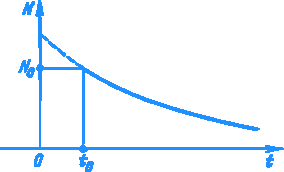
\includegraphics[width=0.6\textwidth]{figures/fig-56.pdf} 
\caption{Graphically depicting radioactive decay of nuclei.}
\label{fig-56}
\end{figure}

\rdr Equation \eqref{nuclear-decay} is a differential equation of type
\eqref{harmonic-osc2} from the preceding dialogue, in which$p = -\dfrac{1}{\tau}$. The initial condition in this case is $N (t_{0}) = N_{0}.$ By using result \eqref{exp-soln} of the preceding dialogue, we immediately obtain
\begin{equation}%
\boxed{
N (t) =N_{0} \, \exp \left( - \dfrac{1}{\tau} (t - t_{0}) \right)}
\label{nuclear-decay-soln}
% eq 2 of 14
\end{equation}

\athr Correct. The formula that you have written, i.e, \eqref{nuclear-decay-soln}, describes the \emph{law of radioactive decay}; we find that this decay is exponential. The number of non-decayed nuclei decreases with time exponentially (\fig{fig-56}).

By taking the logarithm of equality \eqref{nuclear-decay-soln} (using natural logarithms), we obtain
\begin{equation*}%
\ln N(t) = \ln N_{0} - \dfrac{t - t_{0}}{\tau}
\end{equation*}
This yields
\begin{equation*}%
\tau = \dfrac{t - t_{0}}{\ln \dfrac{N_{0}}{N(t)}}
\end{equation*}
The constant $\tau$ is, therefore, such a time interval during which the number of non-decayed nuclei diminishes by a factor of $e$ (i.e. approximately by a factor of 2.7); indeed, in this case $\ln \dfrac{N_{0}}{N(t)} = \ln e = 1$.

\begin{figure}[!ht]%[13]{r}{0.5\textwidth}
\centering
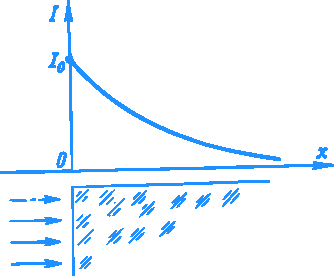
\includegraphics[width=0.6\textwidth]{figures/fig-57.pdf} 
\caption{A light wave propagating through a interface medium.}
\label{fig-57}
\end{figure}

Let us turn now to a different physical problem. Let a light wave with intensity $I_{0}$ be incident perpendicularly at a boundary (the so-called interface) of a medium; the wave propagates through the medium with gradually attenuating intensity. We choose the $x$-axis as the wave propagation direction and place the origin (point $x = 0$) on the interface (\fig{fig-57}). We want to find $I (x)$, that is, the light intensity as a function of the depth of penetration into the medium (in other words, on the path traversed within this medium). We also know that the rate of attenuation at a given point $x$ (i.e. the quantity $-I' (x)$ is proportional to the intensity at this point:
\begin{equation}%
\boxed{
-I' (x) = \eta \, I(x)}
\label{light-absorption}
% eq 3 of 14
\end{equation}

Here $\eta$ is the proportionality factor whose dimension is, obviously, that of inverse length; its physical meaning will be clear somewhat later.

This, therefore, is the formulation of the physical problem.

\rdr It is readily apparent that, as in the preceding case, we deal here with a differential equation of exponential decay. The initial condition is $I (0) = I_{0}$. By using result \eqref{exp-soln} of the preceding dialogue, we obtain
\begin{equation}%
%\boxed{
I (x) = I_{0} \exp (- \eta x)
%}
\label{light-absorption-soln}
% eq 4 of 14
\end{equation}
\athr Formula \eqref{light-absorption-soln} describes \emph{Bouguer's law}, well
known in optics: as light penetrates the matter, its intensity decays exponentially (see \fig{fig-57}).  We readily see that the constant $\eta$ is a quantity inverse to the length along which the light intensity diminishes by a factor of $e$. The constant $\eta$ is called the \emph{linear absorption coefficient}.

Note that results \eqref{nuclear-decay-soln} and \eqref{light-absorption-soln} describe two \emph{different} physical problems from different fields of physics. We describe here two \emph{different physical processes}. Nevertheless, the mathematical nature of these physical processes is the same: both are described by the \emph{same differential equation}.

Let us consider a different physical problem. Assume that a ball with mass $m$, attached to fixed walls by elastic springs, vibrates along the $x$-axis (\fig{fig-58}). The origin $x = 0$ is chosen in the position in which the ball is at equilibrium, that is, half-way between the walls. The motion of the ball is governed by \emph{Newton's second law}:
\begin{equation}%
%\boxed{
ma = F
%}
\label{second-law}
% eq 5 of 14
\end{equation}
where $a$ is acceleration, and $F$ is the restoring force. We assume that
\begin{equation}%
%\boxed{
F= - kx
%}
\label{spring-eqn}
% eq 6 of 14
\end{equation}
where $k$ is the elasticity factor characterizing the elasticity of the spring.
We shall consider the displacement of the ball from the equilibrium position (i.e. the quantity $x$) as a function of time, $x (t)$. This is the function we want to find.

\begin{figure}[!ht]%[13]{r}{0.5\textwidth}
\centering
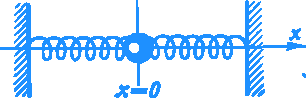
\includegraphics[width=0.6\textwidth]{figures/fig-58.pdf} 
\caption{A mass attached between two elastic springs.}
\label{fig-58}
\end{figure}


We remind the reader that acceleration is the second derivative of a function which describes path as a function of time: $a = x'' (t)$. Consequently, we can rewrite \eqref{second-law}, taking into account \eqref{spring-eqn} in the form
\begin{equation*}%
m x'' (t) + k \, x (t) = 0
\end{equation*}
or
\begin{equation}%
\boxed{
x'' (t) + \dfrac{k}{m} x \, (t) = 0
}
\label{spring-eqn2}
% eq 7 of 14
\end{equation}

\rdr This is a differential equation of type \eqref{harmonic-osc2} of the preceding dialogue provided that $q = \dfrac{k}{m}$.

\athr This means that the general solution must be of the form
\begin{equation}%
%\boxed{
x(t)=A \sin \left( \sqrt{\dfrac{k}{m}} \, t + \alpha \right)
%}
\label{spring-soln}
% eq 8 of 14
\end{equation}

We thus find that the ball in the problem vibrates harmonically around its equilibrium position $x = 0$. The parameter $A$ is, obviously, the \emph{amplitude of vibrations}. The parameter $\alpha$ is called the \emph{initial phase of vibrations}. Recalling relation \eqref{harm-soln7} of the previous dialogue, we conclude that the \emph{period of vibrations} is
\begin{equation}%
%\boxed{
T = 2 \pi \sqrt{\dfrac{m}{k}}
%}
\label{spring-period}
% eq 9 of 14
\end{equation}
Instead of the period $T$, the so-called \emph{angular frequency} $\omega$ is	often used: $\omega=	\dfrac{2 \pi}{T}$.	Formula \eqref{spring-period} yields
\begin{equation}%
%\boxed{
\omega = \sqrt{\dfrac{k}{m}}
%}
\label{spring-period2}
% eq 10 of 14
\end{equation}
By using \eqref{spring-period2}, we rewrite general solution \eqref{spring-soln} in the form
\begin{equation}%
%\boxed{
x(t) = A \sin (\omega t + \alpha)
%}
\label{spring-period2}
% eq 11 of 14
\end{equation}

\rdr And what about the initial conditions in this case? 

\athr Assume that the ball is at rest at $t < 0$. By
setting specific initial conditions at $t = 0$, we choose a method by which vibrations are initiated at the moment $t = 0$. For example, let the initial conditions be given by
relations \eqref{intial-condn3} of the previous dialogue: 
\begin{equation}%
%\boxed{
x(0) = 0,	\quad x'(0) = v_{0}
%}
\label{spring-initial-condn}
% eq 12 of 14
\end{equation}
This means that at the moment $t = 0$ the ball which is at the equilibrium position ($x = 0$) starts moving at a velocity $v_{0}$. According to relation \eqref{harm-soln6} of the previous dialogue, we obtain the following particular solution:
\begin{equation}%
%\boxed{
x (t) = \dfrac{v_{0}}{\omega} \, \sin ( \omega t)	
%}
\label{spring-soln2}
% eq 13 of 14
\end{equation}
Now try to discern the physical meaning of the initial conditions of type \eqref{intial-condn4} of the previous dialogue. 

\rdr These conditions have the form:
\begin{equation}%
%\boxed{
x(0) = x_{0}, \quad x' (0) =0	
%}
\label{spring-soln2}
% eq 14 of 14
\end{equation}
This means that at the initial moment $t = 0$ the ball was displaced from the equilibrium position by $x = x_{0}$ and let go. The corresponding particular solution, following from relation \eqref{harm-soln7} of the previous dialogue, takes the form
\begin{equation}%
%\boxed{
x (t) = x_{0} \cos \, (\omega t)
%}
\label{spring-soln2}
% eq 15 of 14
\end{equation}

\athr
\athr In the first case we thus initiate vibrations by imparting the initial velocity $v_{0}$ to the ball at the equilibrium position (in this case the amplitude $A$ of vibrations is $\dfrac{v_{0}}{\omega}$, and the initial phase $\alpha$, can be set equal to zero, in 0) accordance with \eqref{spring-soln2}). In the second case the vibrations are initiated by displacing the ball from the equilibrium position by $x_{0}$ and then letting it go (in this case $A= x_{0}$, and the initial phase a can be set equal to $\dfrac{\pi}{2}$, in accordance with \eqref{spring-soln2}. 

\rdr Could we consider a case in which at $t = 0$ the ball is displaced from the equilibrium position by $x_{1}$ and simultaneously given an initial velocity $v_{1}$?

\athr Of course, this is one of the possible situations. \fig{fig-59} shows four vibration modes (four particular solutions) corresponding to four different initial conditions

(four different methods of starting the vibrations of the ball):
\begin{enumerate}[label=\protect\circled{\arabic*}]
\item $x(0) =0, \,\, x' (0) = v_{0}$; in this case $A = \dfrac{v_{0}}{\omega}, \,\, \alpha = 0$.
\item $x(0) =x_{0}, \,\, x' (0) = 0$; in this case $A = x_{0}, \,\, \alpha = \dfrac{\pi}{2}$.
\item $x(0) =x_{1}, \,\, x' (0) = v_{1}$; (the initial velocity imparted to the ball has the same direction as the initial displacement); in this case $A = A_{1}, \,\, \alpha = \alpha_{1}$ (see the figure).
 \item $x(0) =x_{1}, \,\, x' (0) = -v_{1}$; (the initial velocity imparted to the ball has the direction opposite to that of the initial displacement); in this case $A = A_{1}, \,\, \alpha = \pi - \alpha_{1}$ (see the figure).
\end{enumerate}
As follows from relation \eqref{harm-soln3} of the preceding dialogue,
\begin{equation}%
%\boxed{
 A_{1} = \sqrt{ x_{1}^{2} + \left( \dfrac{v_{1}}{\omega} \right)^{2}}
 %}
\label{spring-soln3}
% eq 16 of 14
\end{equation}
and according to \eqref{spring-period2},
\begin{equation}%
%\boxed{
 \alpha_{1} = \arctan \left( \dfrac{x_{1} \omega}{v_{1}} \right)
 %}
\label{spring-soln4}
% eq 17 of 14
\end{equation}

\rdr I notice that by fixing specific initial conditions (in other words, by initiating the vibrations of the ball by a specific method), we predetermine the amplitude and initial phase of the vibrations.


\begin{figure}[!ht]%[13]{r}{0.5\textwidth}
\centering
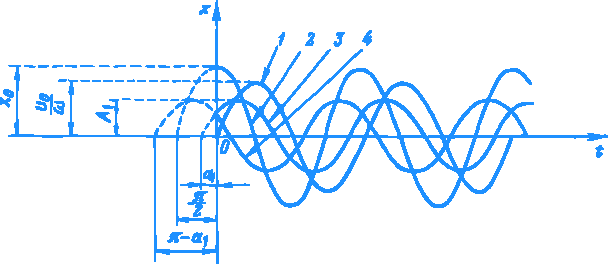
\includegraphics[width=\textwidth]{figures/fig-59.pdf} 
\caption{Four vibration modes (four particular solutions) corresponding to four different initial conditions.}
\label{fig-59}
\end{figure}

\athr Precisely. This is clearly shown in \fig{fig-59}. By the way, the same figure shows that the period of vibrations (their frequency) remains constant regardless of the initial conditions.

To summarize, we note that a harmonic oscillation is characterized by three parameters (see \eqref{spring-period2}) the amplitude $A$, initial phase $\alpha$, and frequency $\omega$, The first two parameters are determined by the choice of initial conditions, and the last parameter is independent of them.

The above-described process of vibrations is one of the \emph{mechanical} processes. Let us turn now to a process of an essentially different physical nature. We shall analyze the motion of electric charges in a circuit consisting of a capacitor with capacitance $C$ and a coil with inductance $L$ (\fig{fig-60}).

\begin{figure}[!ht]%[13]{r}{0.5\textwidth}
\centering
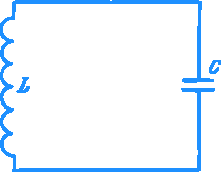
\includegraphics[width=0.4\textwidth]{figures/fig-60.pdf} 
\caption{Analysing electrical oscillations in a circuit with a capacitor and an inductor.}
\label{fig-60}
\end{figure}

Let the capacitor plates have a charge $Q(t)$ at a moment $t$; correspondingly, the potential difference between the capacitor plates will be $\dfrac{Q(t)}{C}$. If the current in the circuit at the moment $t$ is $i (t)$, then the potential difference generated in the coil is $-L i' (t)$. We know that it must be balanced out by the potential difference across the capacitor plates:
\begin{equation}%
%\boxed{
- L i' (t) = \dfrac{Q(t)}{C}	
 %}
\label{lc-ckt}
% eq 18 of 14
\end{equation}
Let us differentiate relation \eqref{lc-ckt}. This gives
\begin{equation}%
%\boxed{
-Li''(t)=  \dfrac{Q'(t)}{C}	
 %}
\label{lc-ckt}
% eq 19 of 14
\end{equation}
Now we shall take into account that
\begin{equation*}%
Q'(t) = i(t)
\end{equation*}
(current intensity, or simply current, is the rate of change of charge). As a result, equation \eqref{lc-ckt} can be rewritten in the form:
\begin{equation*}%
-L i'' (t) = \dfrac{1}{C} i (t)
\end{equation*}
or
\begin{equation}%
\boxed{
i'' (t) + \dfrac{1}{LC} i (t) = 0
 }
\label{lc-ckt2}
% eq 20 of 14
\end{equation}
The resultant differential equation is quite familiar, isn't it?

\rdr This is a differential equation of type \eqref{harmonic-osc2}
of the preceding dialogue provided that $q = \dfrac{1}{LC}$. We con-
clude, therefore, that the process in the circuit is harmonic. 

\athr Note, however, that the process is not that of mechanical vibrations of a ball attached to springs but the process of \emph{electromagnetic oscillations} in an electric circuit. 

\rdr As  $q = \dfrac{1}{LC}$ and using relation \eqref{harm-soln7} of the previous dialogue, we obtain a relation for the period of electromagnetic oscillations in the circuit:
\begin{equation}%
%\boxed{
T =  2 \pi \sqrt{LC}
 %}
\label{lc-ckt-period}
% eq 21 of 14
\end{equation}
The general solution of equation \eqref{lc-ckt2} is then
\begin{equation}%
%\boxed{
i (t) = A \sin \left( \frac{1}{\sqrt{LC}} t + \alpha \right) 
 %}
\label{lc-ckt-soln}
% eq 22 of 14
\end{equation}

\athr Absolutely correct. The two physical processes, namely, the \emph{mechanical vibrations} of a ball attached to springs and the \emph{electromagnetic oscillations} in a circuit, are \emph{mathematically similar}. They are described by the same differential equation. Otherwise you couldn't write, nearly automatically as you did, the period of oscillations (formula \eqref{lc-ckt-period} and the general solution (formula \ref{lc-ckt-soln}).

In our dialogues we have discussed only two (and rather simple) types of differential equations: those of exponential growth (decay) and of harmonic oscillations. And we have illustrated them with a number of physical processes of very different kind.

\rdr I guess that the list of different differential equations, and certainly the list of physical processes described by these equations, could be substantially enlarged.

\athr No doubt. This concludes our discussion of differential equations. I want to note in conclusion that differential equations are widely applied not only in physics but in chemistry, biology, cybernetics, sociology, and other fields of science as well.